%----------------------------------------------------------------------------------------
%	PACKAGES AND DOCUMENT CONFIGURATIONS
%----------------------------------------------------------------------------------------
\documentclass[11pt]{article}
\usepackage{amsmath} % Required for some math elements
\usepackage{hyperref} 
\usepackage[usenames,dvipsnames]{xcolor}
\usepackage{lipsum} 
\usepackage{cite}
\usepackage{graphicx} % Required for the inclusion of images
\usepackage{algorithmic}
\usepackage{array}
\usepackage{bookmark}
\usepackage{listings}
\usepackage{amssymb}
\usepackage{enumitem}
\usepackage[margin=24mm]{geometry}
\usepackage[caption=false, font=footnotesize]{subfig}
\usepackage{multirow}
\usepackage[active,tightpage]{preview}

\renewcommand{\PreviewBorder}{1in}
\newcommand{\Newpage}{\end{preview}\begin{preview}}

\newlist{steps}{enumerate}{1}
\setlist[steps, 1]{label = Step \arabic*:}

\hypersetup{ %color attributes of citation, link, etc.
    colorlinks=true,
    linkcolor=blue,
    filecolor=gray,      
    urlcolor=blue,
    citecolor=blue,
}

 
\lstdefinelanguage{VHDL}{
   morekeywords=[1]{
     library,use,all,entity,is,port,in,out,end,architecture,of,
     begin,and,or,Not,downto,ALL
   },
   morekeywords=[2]{
     STD_LOGIC_VECTOR,STD_LOGIC,IEEE,STD_LOGIC_1164,
     NUMERIC_STD,STD_LOGIC_ARITH,STD_LOGIC_UNSIGNED,std_logic_vector,
     std_logic
   },
   morecomment=[l]--
}
\definecolor{keyword}{rgb}{0,0.3,0.7}
\definecolor{STD}{rgb}{0.9,0.0,0.7}
\definecolor{comment}{rgb}{0.0,0.6,0.1}

\lstdefinestyle{vhdl}{
   language     = VHDL,
   basicstyle   = \footnotesize\ttfamily,
   keywordstyle = [1]\color{keyword}\bfseries,
   keywordstyle = [2]\color{STD}\bfseries,
   commentstyle = \color{comment}
   breaklines=true,                % sets automatic line breaking
   tabsize=3		                   % sets default tabsize to 2 spaces
}


\newcommand{\matlab}{\textsc{Matlab }} %very important and totally necessary addition

\newcommand\Item[1][]{%
  \ifx\relax#1\relax  \item \else \item[#1] \fi
  \abovedisplayskip=0pt\abovedisplayshortskip=0pt~\vspace*{-\baselineskip}}
  %----------------------------------------------------------------------------------------
%	DOCUMENT INFORMATION
%----------------------------------------------------------------------------------------
 
\title{ECEN302 : Embedded Systems \\ Lab 2 Submission}
\author{Daniel Eisen : 300447549}
\date{\today}

\begin{document}
\begin{preview}
\maketitle
%----------------------------------------------------------------------------------------
%	DOCUMENT CONTENT
%----------------------------------------------------------------------------------------
\section{Objectives}
When designing in VHDL (or Verilog etc) the are various methods/approaches in obtaining the same results. In this lab we explore multiple ways of structuring a VHDL module, using the example of a MUX in multiple configurations. This gave a good idea of how to use/implement standard module structures and the pros/cons of their use cases.


\section{Methodology}
        \subsection{Dataflow Modelling}
        Firstly we used dataflow modelling to implement a 1bit and a 2bit 2-to-1 multiplexer. This method is based mainly around concurrent assignment to either the ports directly, or an intermediate signal. I found that this method of structuring a module is particularly good operations are around getting an input signal(s) and a known output is wanted, ie the data is known and the "component" makeup doesn't matter. Ie this is good for a simple module that isn't combining multiple pre-existing modules together.

        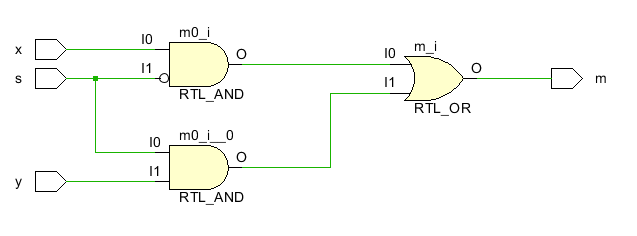
\includegraphics[width=\textwidth]{res/part1/part1_1Wmux2_1.PNG}
        Implementing a 1-bit wide 2 to 1 mux with dataflow is quite simple, with the output port being determined with a single line of logic.\\

        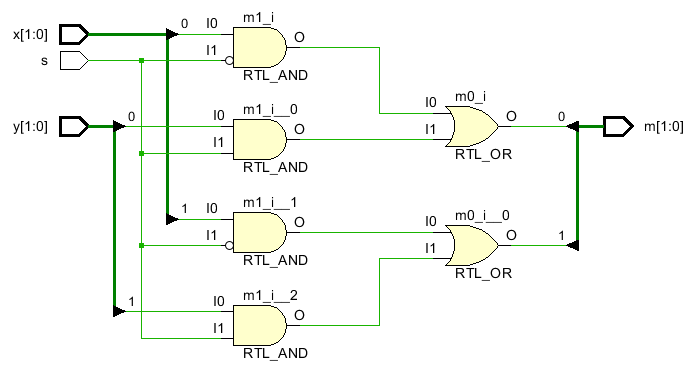
\includegraphics[width=\textwidth]{res/part1/part1_2Wmux2_1.PNG}
        Extending this to a bus input only required a second line for the second bit.\\

        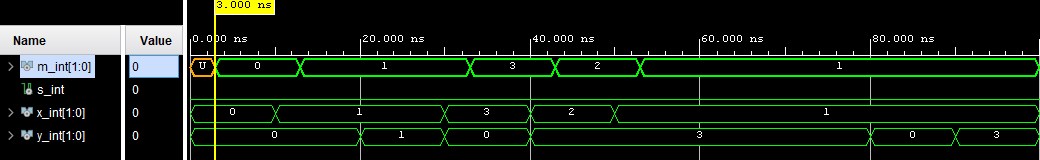
\includegraphics[width=\textwidth]{res/part1/part1_sim.PNG}
        When the source value changes it is evaluated, but the result can be delayed from being assigned to its destination. This is seen in the simulation above (3ns).\\ 

        \subsection{Structural Modelling}
        When the design more fits connecting multiple pre-existing components to defined the overall functionality of the circuit, structural modelling can be used to instantiate these components (whether they are other modules or just gate primitives).

        In this section the previous design of the 2bit 2-to-1 with structural modelling. Building it out of individual logic gate primitives, this involves instantiating each element type (and, not, or), port mapping them, and creating each part and connecting them via internal signals. For this particular use case this is far too tedious, and probably the wrong application of the structural modelling approach, as for such a simple more data oriented design the code becomes non-representatively long and complex/unreadable.

        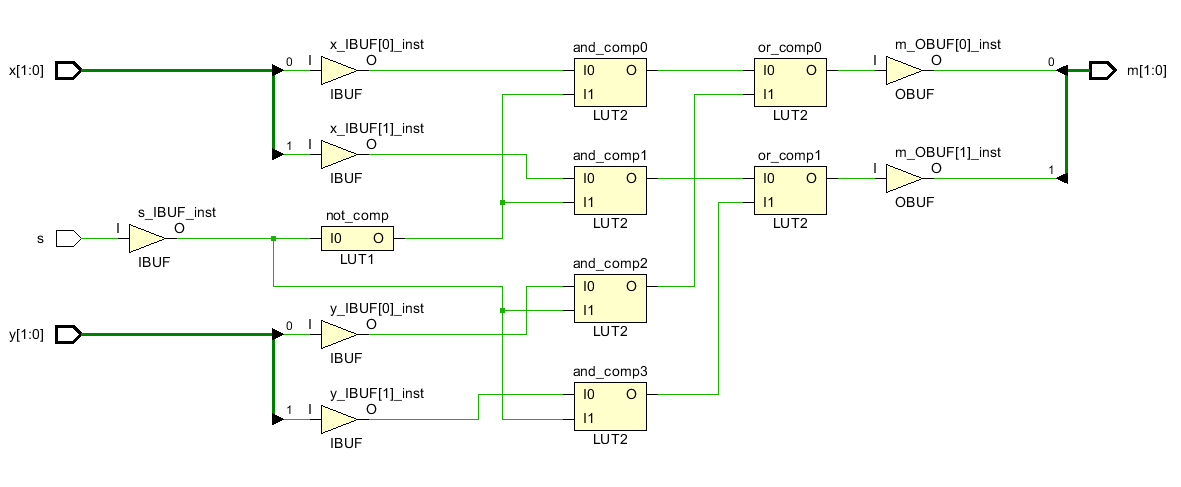
\includegraphics[width=\textwidth]{res/part2/part2_2bitmux.PNG}
        Above is the result of the structural modelling approach.
        \subsection{Behavioural Modelling}
        In the dataflow example multiple port assignment is down concurrently, in the Behavioural model a process is defined for a specific function and the statements are then executed sequentially. When doing this with the muxs it is displayed as a mux element before synthesis, but after synthesis can either be implemented in a concurrent or sequential circuit. If this allows for the use of \texttt{if,else,then} etc.
        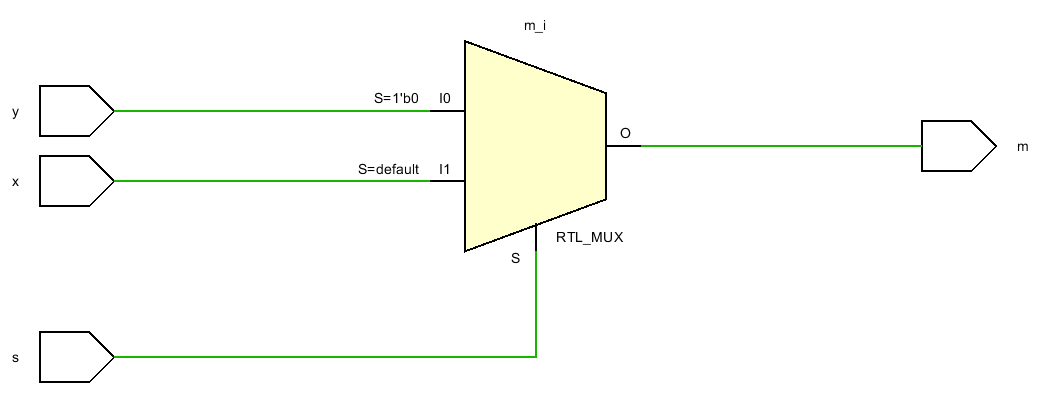
\includegraphics[width=\textwidth]{res/part3/part3_1bitmux.PNG}
        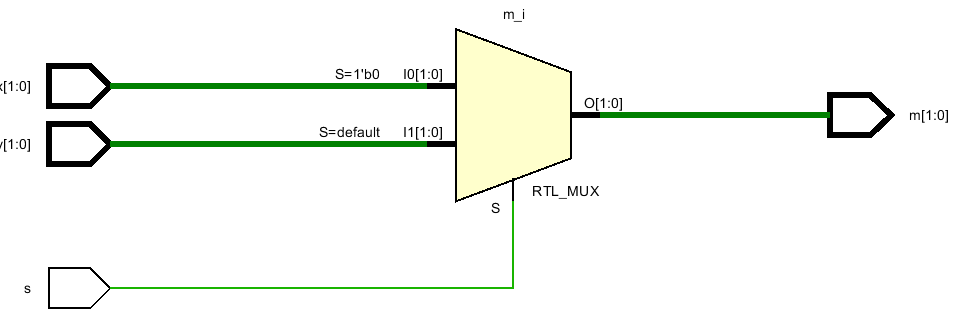
\includegraphics[width=\textwidth]{res/part3/part3_2bitmux.PNG}
        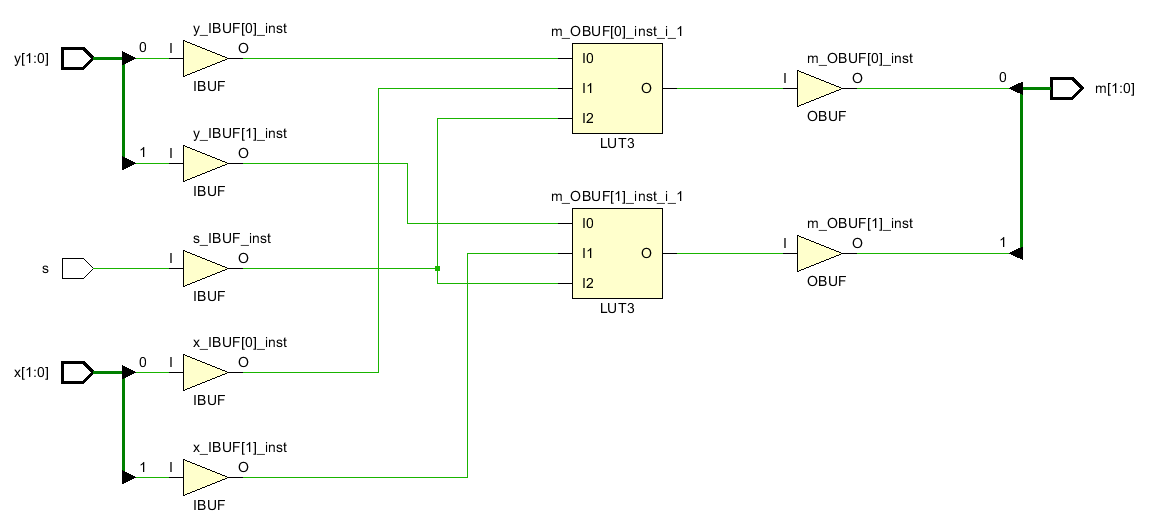
\includegraphics[width=\textwidth]{res/part3/part3_2bitmux_synth.PNG}
        \subsection{Mixed-Design Modelling}
        To bring it all together in a more useful application of the modelling methods, the dataflow modelled 2-to-1 mux was imported into the project and used to build a 3-to-1 mux. In this case, the mux\_2bit\_2\_1 was imported and mapped, a intermediate output signal created to feed the first out into the second, and the circuit functionality/connections defined using structural modelling. This is an example of good application of the structural method of using smaller modules to construct a more complex function. 
        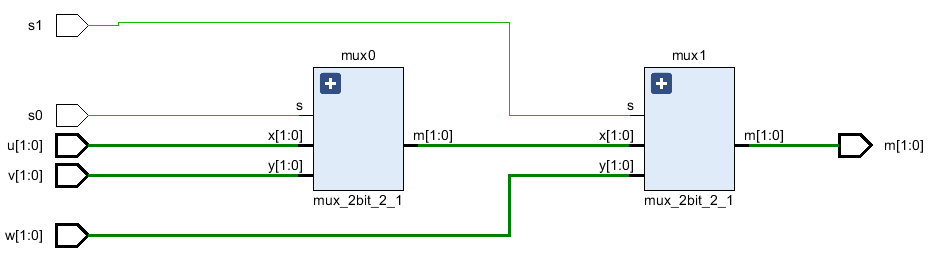
\includegraphics[width=\textwidth]{res/part4/schem0.PNG}
        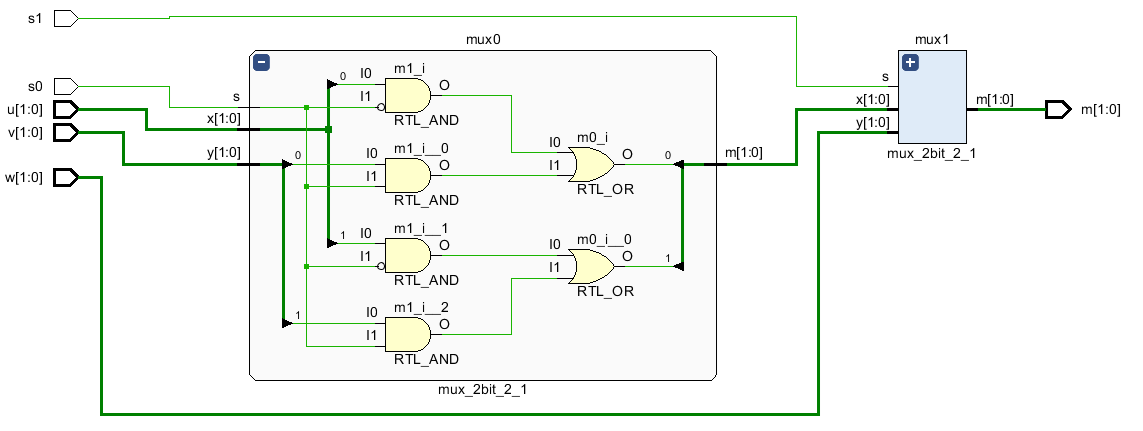
\includegraphics[width=\textwidth]{res/part4/schem1.PNG}
        \subsection{BCD to 7 segment}
        In a previous the 7 segment display was used. This time a config word was used to set the use a specific displayed digit by setting/clearing the anodes. So the display of the first digit, its anode is cleared and the rest set high. \texttt{an <= "11111110"}.
        To speed up the process the previously written BCB to 7 segment encoding lookup table (select statement) was used.

\section*{Appendix}

\subsection*{Part 1 - Dataflow}
\subsubsection*{Mux}
\begin{center}
  \fbox{\lstinputlisting[language=VHDL]{res/part1/lab_2_2_1.vhd}}
  \vspace*{32px}
\end{center}

\subsubsection*{Two Bit Mux}
\begin{center}  
  \fbox{\lstinputlisting[language=VHDL]{res/part1/mux_2bit_2_1.vhd}}
  \vspace*{32px}
\end{center}

\subsubsection*{Mux delay}
\begin{center}
  \fbox{\lstinputlisting[language=VHDL]{res/part1/mux_2bit_2_1_delay.vhd}}
  \vspace*{42px}
\end{center}

\subsection*{Part 2 - Structural}
\subsubsection*{Two Bit Mux}
\begin{center}  
  \fbox{\lstinputlisting[language=VHDL]{res/part2/lab_2_3_1.vhd}}
  \vspace*{42px}
\end{center}

\subsection*{Part 3 - Behavioural}
\subsubsection*{Mux}
\begin{center}
  \fbox{\lstinputlisting[language=VHDL]{res/part3/lab_2_4_1.vhd}}
  \vspace*{32px}
\end{center}

\subsubsection*{Two Bit Mux}
\begin{center}  
  \fbox{\lstinputlisting[language=VHDL]{res/part3/lab_2_4_2.vhd}}
  \vspace*{42px}
\end{center}

\subsection*{Part 4 - Mixed}
\subsubsection*{3 to 1 Mux}
\begin{center}
  \fbox{\lstinputlisting[language=VHDL]{res/part4/mux_3_to_1.vhd}}
  \vspace*{32px}
\end{center}

\subsection*{DCD to 7 seg}
\begin{center}  
  \fbox{\lstinputlisting[language=VHDL]{res/part4/dcd_7seg.vhd}}
  \vspace*{42px}
\end{center}
  
  
\end{preview}
\end{document}